\pagestyle{empty}
\cleardoublepage
\pagestyle{fancy}

\chapter{Revisão da Literatura}\label{chap:revisao}

Neste capítulo apresentamoas a revisão bibliográfica das teorias utilizadas neste estudo. 


\section{Regressão Linear}\label{sec:regressao_linear}

Fenômenos da natureza, ou aqueles provocados pela ação do homem, podem ser estudados decompondo-os em variáveis numéricas ou categóricas, a fim de observar as relações entre elas e, possivelmente, identificar padrões comportamentais ou estimar resultados com base em suposições. Essas relações podem ser determinadas elencando-se um ou mais dessas variáveis como as variáveis de interesse a serem expressas em função das demais variáveis restantes.  Ao longo desse estudo denominaremos as variáveis de interesse por \textbf{variáveis dependentes}, cujo nome apropriadamente indica uma relação de dependência com as demais variáveis, denominadas \textbf{variáveis independentes}, \cite[p.2]{Andersen}. Como o escopo desse estudo limita-se a apenas uma variável independente, representamos uma observação qualquer dessa variável por $ y $ e as respectivas $ n $ variáveis independentes pelo vetor $ x = (x_1, x_2, ..., x_n) $.  As matrizes $ Y_{m,1} $, $ X_{m,n} $ representam o conjunto de $ m $ observações das variáveis dependente e independentes, respectivamente, sendo uma determinada observação $ i $ indicada por $ y_i,\text{ }x_i,\text{ }i\in \{1,2,...,m\} $ e uma determinada variável independente $ j $ por $ x_{j}\text{ }, j\in\{1,2,...,n\} $. Finalmente, $ x_{ij} $ representa uma observação específica $ i $ da variável independente $ j $.


Um dos objetivos da compreensão de um fenômeno é a capacidade de estimar um valor da variável dependente, indicado por $ \hat{y} $, a partir de uma nova observação $ x \notin X$, esperando-se seguir as relações naturalmente presentes em $ Y $ e $ X $. Quando $ \hat{y} $  pode assumir um valor contínuo, $ \hat{y} \in \mathbb{R} $, chamamos a essa estimação de \textbf{Regressão} \cite[p.3]{Bishop}, \cite[p.4]{Hastie}. A estimação de variáveis dependentes categóricas, aquelas que representam a pertinência a um determinado conjunto, é chamado \textbf{Regressão Logística} e não é escopo desse estudo. 


\cite[p.44]{Hastie},\cite[p.138]{Bishop} e \cite[p.127]{Murphy} definem \textbf{Regressão Linear} a classe de modelos cuja função de regressão da variável dependente $ \hat{y} $ é uma combinação linear dos parâmetros $ \beta_i \in \mathbb{R} $ :

\begin{equation}\label{eq:reg_linear}
\hat{y} = \beta_0 + \beta_1x_1 + ... + \beta_nx_n
\end{equation}

Segundo \cite[9-11]{Andersen}, para os casos em que $ x_j $ é categórica, $ x_j \in {c_1,c_2,...,c_k} $, não a utilizamos diretamente no modelo, mas a substituímos por variáveis \textbf{dummy}\footnote{Sem tradução direta para a Língua Portuguesa.}, assim denominadas para representar a pertinência à categoria identificada em  $ x_j $. Tal substituição é feita criando-se $ k $ variáveis indicadoras para as $ k+1 $ categorias possíveis de $ x_j $:

\begin{equation}
I_{1,...,k}(x_j)=
	\begin{cases}
		1, \text{se }x_j = c_r \\
		0, \text{senão}
	\end{cases}
\end{equation}



O coeficiente $ \beta_0 $ na equação \ref{eq:reg_linear} representa um deslocamento fixo do modelo, valor a ser assumido para o caso em que $ \forall j: x_j = 0 $, denominado  \textit{bias}\footnote{Não há tradução clara do significado desse termo conforme \cite[p.138]{Bishop} para a Língua Portuguesa.}. Por conveniência, assumimos uma nova variável independente $ x_0=1 $, fazendo o conjunto de variáveis independentes ter dimensões $ X_{m,n+1} $, com o propósito de reduzir a equação \ref{eq:reg_linear} para a forma:

\begin{equation}\label{eq:reg_linear_bishop}
\hat{y} = \sum_{j=0}^{n}\beta_j x_j
\end{equation}

Entretanto os parâmetros $ \beta $ são desconhecidos e também precisam ser estimados. Podemos fazê-lo a partir de um subconjunto das observações $ Y $ e $ X $, a quem denominamos \textbf{conjunto de treinamento} \cite[p.4]{Bishop}, \cite[p.1]{Hastie}. A utilização dos valores atuais $ Y $ de forma a permitir uma avaliação da eficiência da estimação de $ \beta $ classifica esse tipo de aprendizado como \textbf{supervisionado} \cite[p.2]{Hastie}. Reciprocamente, aprendizados \textbf{não supervisionados} são aqueles que procuram identificar estruturas em $ X $ e não dependem de $ Y $ para avaliar o aprendizado.


Segundo \cite[p.12]{Hastie}, um dos métodos mais populares utilizado para a estimação de $ \beta $, conhecido como \textbf{Método dos Mínimos Quadrados}\footnote{Do inglês \textit{Least Squares}, tradução nossa.}, consiste em minimizar a soma dos quadrados dos erros residuais $ \epsilon_i = y_i - \hat{y}_i $: 

\begin{equation}\label{eq:least_squares}
\hat{\beta} = \argmin_\beta \sum_{i=1}^{m} (\sum_{j=0}^{n}\beta_j x_{ij} - y_{i})^2
\end{equation}



Importante notar que o erro residual não é a distância euclidiana entre $ y $ e $ \hat{y} $, mas tão somente a diferença escalar entre as duas variáveis, como pode ser visto na \cref{fig:bishop_least_square_intuition}.

\begin{figure}[h!]
\centering
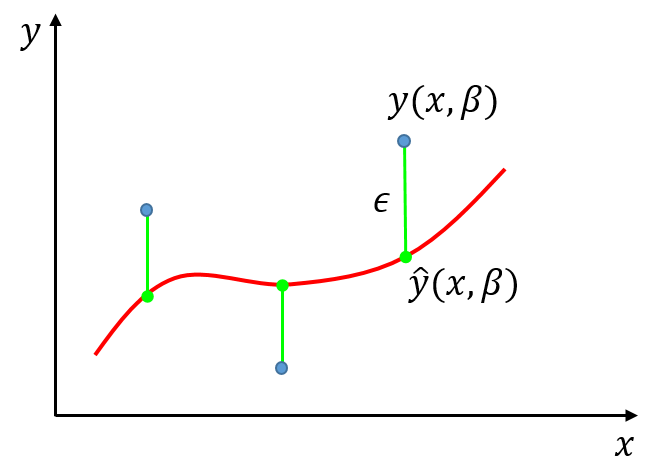
\includegraphics[width=0.5\linewidth]{img/intuicao_epsilon}
\caption[Intuição do método Mínimos Quadrados.]{Intuição do método Mínimos Quadrados. Fonte: \cite[p.6]{Bishop}, adaptado.}

\label{fig:bishop_least_square_intuition}
\end{figure}

A equação \ref{eq:least_squares} pode ser descrita em forma matricial, onde denominamos $ RSS(\beta) $ a \textit{Soma dos Resíduos Quadrados}\footnote{Do inglês \textit{Residual Sum of Squares, RSS} \cite[p.12]{Hastie}}:

\begin{align}\label{eq:ols_matrix}
RSS(\beta) &= \sum_{i=1}^{m} (\sum_{j=0}^{n}\beta_j x_{ij} - y_{i})^2 \nonumber\\
&= \sum_{i=1}^{m} (\beta^Tx_i - y_i)^2 \nonumber\\
&= (Y-X\beta)^T(Y-X\beta)
\end{align}

Derivando-se \eqref{eq:ols_matrix} com com respeito a $ \beta $ temos:
\begin{align}
0=X^T(y-X\beta)
\end{align} 

Se $ X^TX  $ for não singular, então a solução única é dada por:

\begin{align}\label{eq:hat_beta}
\hat{\beta} = (X^TX)^{-1}X^TY
\end{align} 

Se $ X^TX $ for singular, então a equação \ref{eq:hat_beta} admite mais de uma solução, o que indica interdependência linear entre as variáveis $ X $. Deparamo-nos então com uma das primeiras premissas para a utilização do Método de Mínimos Quadrados para estimação de $ \beta $, que é a independência linear entre as variáveis independentes.


Finalmente, de posse de uma nova observação $ z \notin X $ podemos estimar o valor da variável dependente $ \hat{y}(z) $ com:
\begin{align}
\hat{y}(z) = z^T\beta
\end{align}


%Estendemos a equação acima adicionando o erro residual $ \epsilon $, que é a diferença numérica entre o valor real $ y $ e o valor estimado $ \hat{y} $ para uma determinada observação $ (y,x) $ em função de $ \beta $  \cite[p.19]{Murphy} :
%
%
%\begin{align}\label{eq:reg_linear_murphy}
%y - \hat{y} = \epsilon \nonumber \\
%y = \hat{y} + \epsilon \nonumber \\
%y = \sum_{j=0}^{n}\beta_j x_j + \epsilon 
%\end{align}
%



\cite[p.140-143]{Bishop} e \cite[p.178-180]{Andersen} demonstram que o Método dos Mínimos Quadrados é derivado da Estimativa por Máxima Verossimilhança sob a premissa de que o erro residual $ e_i = y_i - \hat{y_i} $ segue uma distribuição Normal.

Sob determinadas condições das escolhas das variáveis independentes em $ X $ e o número $ m $  de observações, podemos incorrer em um problema denominado \textbf{Sobreajuste}\footnote{Do inglês \textit{Overfitting}, tradução nossa.}\cite[p.]{Bishop}.\todo{Renato:Devo explicar matematicamente a causa de overfitting que envolve demonstração estatística bayesiana???} que implica na estimação de $ \hat{\beta} $ fazer $ \hat{y}(x) $ demasiadamente bem de $ y(x) $ para $ x \in X $ mas não aproximar bem em novas observações $ x \notin X $. \cite[p.4-9]{Bishop} ilustra esse problema com uma aplicação bem simples de Regressão Linear que é ajustar uma curva polinomial de ordem $ M $, $ \hat{y} = \sum_{i=0}^M \hat{\beta}x^i$, a partir de dados gerados pela função $ y = \sin(x) $, com um ruído aleatório aplicado. Nesse exemplo em que temos apenas uma variável em $ X $, propomos a construção de novas variáveis  $ x^2, x^3, ..., x^M $. Importante notar que essas novas variáveis não apresentam dependência linear com $ x $, respeitando a premissa para que $ X^TX $ seja não singular. 


Vê-se que na \cref{fig:bishop_overfitting} que conforme $ M $ aumenta, o polinômio resultante aproxima-se a $ x $ até que para $ M=9 $ o polinômio passa exatamente exatamente sobre cada um dos dados originais mas distanciará de novas observações. 

\begin{figure}[h!]
\centering
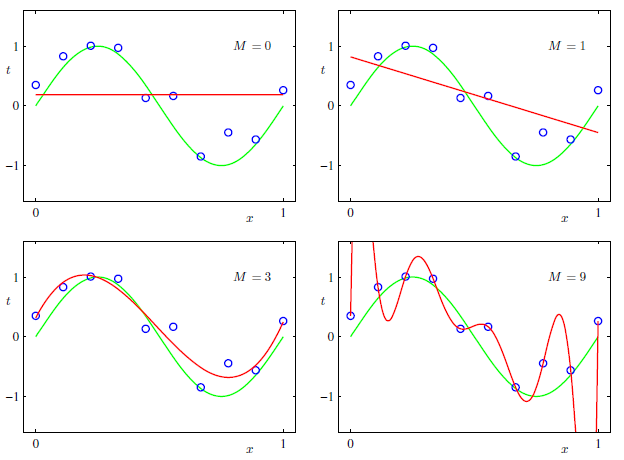
\includegraphics[width=1\linewidth]{img/bishop_overfitting}
\caption[Exemplo de sobreajuste.]{Exemplo de sobreajuste. Fonte: \cite[p.7]{Bishop}, adaptado.}
\label{fig:bishop_overfitting}
\end{figure}

De fato, a definição de sobreajuste apresentada por \cite[p.67, adaptado]{Mitchell} diz:

\begin{quotation}
Given a hypothesis space $ H $, a hypothesis $ \hat{y} \in H $ is said to overfit the training data if there exists some alternative hypothesis $ \hat{y}' \in H $, such that $ \hat{y} $ has smaller error than $ \hat{y}' $ over the training examples, but $ \hat{y}1 $ has a smaller error than $ \hat{y} $ over the entire distribution of instances.
\end{quotation}

Tal definição é empiricamente demonstrada na \cref{fig:bishop_overfitting} em que notamos que para $ M=3 $ a soma dos erros residuais para novas observações será menor do que para $ M=9 $.

Podemos verificar o sobreajuste de uma regressão medindo gráfica e numericamente o comportamento de uma medida de performance da capacidade de generalização de $ \hat{y} $. Usualmente utiliza-se  a \textit{Raiz do Erro Médio Quadrático}\footnote{Do inglês \textit{Root Mean Square Error}, \textit{RMSE}, tradução nossa. Manteremos a sigla em inglês \textit{RMSE} por conveniência.} para esse objetivo,  que é uma extensão da equação \ref{eq:least_squares} definida como \cite[p.7, adaptado]{Bishop}:

\begin{equation}
RMSE = \sqrt{\dfrac{\sum_{i=1}^{m} (\hat{y}-y)^2}{n}}
\end{equation} 

A divisão por $ n $ nos permite comparar diferentes tamanhos de conjuntos de treinamento e a raiz quadrada por sua vez garante que a $ RMSE $ seja medida na mesma escala e unidade da variável dependente $ y $ \cite[p.7]{Bishop}. 

Entretanto, de nada adianta escolher os parâmetros cuja $ RMSE $ seja mínima utilizando o próprio conjunto de treinamento para avaliação da performance pois desta forma estaremos justamente forçando o sobreajuste. Essa situação é resolvida pela técnica da \textbf{Validação Cruzada} separando os conjuntos de observações $ Y $ e $ X $ em dois subconjuntos distintos, um para treinamento, a ser denotado por $ Y_t $ e $ X_t $, e outro para validação, denotados como $ Y_v $ e $ X_v $ \cite[p.32]{Bishop}.                                                                                                             

A \cref{fig:bishop_overfit_error} demonstra a importância da Validação Cruzada na avaliação da performance da generalização de $ \hat{y} $ para novas observações. Continuando com o exemplo do ajuste de um polinômio de ordem  $ M $, calculamos a raiz do erro médio quadrático, $ RMSE $, para cada $ M $, sobre o próprio conjunto de treinamento e sobre um conjunto reservado de verificação. À medida que $ M $ aumenta a performance melhora em ambos, mas para $ M=9 $ fica claro o sobreajuste quando avaliado sobre o próprio conjunto de treinamento e seu impacto na performance sobre o conjunto de verificação. Um efeito prático do sobreajuste sobre os coeficientes $ \beta $ é esses assumirem valores abusolutos expressivos, como pode ser visto no lado esquerdo da \cref{fig:bishop_overfit_error}.

\begin{figure}[h!]
\centering
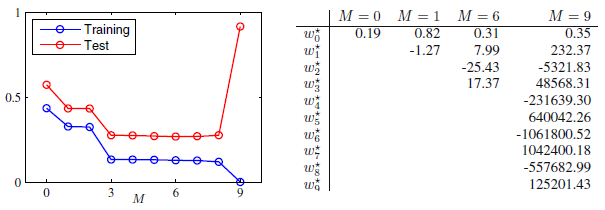
\includegraphics[width=1\linewidth]{img/bishop_overfit_error}
\caption[Intuição do sobreajuste (overfitting)]{Intuição do soreajuste (overfitting) para a estimação de uma função polinomial em $x$. Fonte:\cite[p.8]{Bishop}, adaptado.}
\label{fig:bishop_overfit_error}
\end{figure}


% % % % % % % % % % % % % % % % % % % % % % % % % % % % % % % % % % % % % % % % % % % % % % % % % % % % %
%% EXPLICAÇÃO DO OVERFIT COM BASE NO MODELO BAYESIANO.
%\cite[p.162,p.20]{Bishop,Murphy} esclarecem que o erro residual $ \epsilon $ assume uma distribuição Normal, ou Gaussiana\footnote{Em homenagem ao matemático alemão Gauss(1777-1855): \url{http://en.wikipedia.org/wiki/Carl_Friedrich_Gauss}}, com desvio padrão $ \mu =0 $ e precisão $ \beta = 1/{\sigma^2} $, onde $ \sigma_{2} $ é a variância do conjunto de treinamento $ T $. Assim, a estimação de $ w $ por Mínimos Quadrados, que procura minimizar $ \epsilon $, pode ser interpretada como uma função de máxima verossimilhança:

%\begin{equation}
%p(y|x,w,\beta) = \mathcal{N}(\hat{y}|y(x,w),\beta^{-1})
%\end{equation}
% % % % % % % % % % % % % % % % % % % % % % % % % % % % % % % % % % % % % % % % % % % % % % % % % % % % %

Em função da expressiva magnitude que os coeficientes $ \hat{\beta} $ podem alcançar devido ao sobreajuste, uma alternativa é aplicar sobre a estimação de $ \beta $ uma penalidade proporcional ao crescimento absoluto dos próprios coeficientes, conhecido como \textbf{Regularização}\footnote{Do inglês \textit{Regularization}, tradução nossa.} \cite[p.10,144-147]{Bishop} ou \textbf{Métodos de Encolhimento}\footnote{Do inglês \textit{Shrinkage Methods}, tradução nossa.} \cite[p.61-69]{Hastie}. Abaixo apresentamos a estimação de $ \beta $ com uma penalização denominada \textit{Ridge} \cite[p.63]{Hastie}:

\begin{equation}
\hat{\beta} = \argmin_{\beta} \bigg(  \sum_{i=1}^{m}(y_i - \beta_0 - \sum_{j=1}^{n} \beta_jx_{ij})^2 + \lambda \sum_{j=1}^{n} \beta_{j}^2 \bigg)
\end{equation}

O parâmetro $ \lambda $ controla o grau de penalidade a ser aplicado estimação de $ \beta $. Quanto maior $ \lambda $, maior será a penalidade aplicada, limitando proporcionalmente o crescimento absoluto de $ \beta $. Uma penalidade excessiva pode inverter totalmente o objetivo da regularização e causar o chamado \textit{subajuste}\footnote{Do inglês \textit{Underfitting}, tradução nossa.}, cuja consequência também é a perda de generalização de $ \hat{y} $ para novas observações, inclusive para o próprio conjunto de treinamento \cite[p.38]{Andersen}. 

\iffalse
\section{Análise Exploratória de Dados}

Antes de larçarmo-nos à investigação das relações entre $ Y $ e $ X $, seja por Regressão Linear ou qualquer outro método de inferência, é fundamental conhecer as variáveis observadas individualmente a fim de obter \textit{insights} sobre suas estruturas e identificar possíveis \textit{outliers} e outras anomalias. Tal objetivo é alcançado por uma variedade de técnicas conhecida como \textbf{Análise Exploratória de Dados} \cite{NIST}. 

\fi



\iffalse


\section{Aprendizagem por Máquinas}\label{sec:aprendizagem_maquinas}

Supondo-se que temos uma quantidade razoável de observações $ (y,x)  $, talvez não seja possível, ou quiçá desinteressante, determinar $ F $ analiticamente, mas recorrer a métodos numéricos que possam ser executados por computadores para estimar um modelo que se aproxime de $ F $, a fim de que seja possível encontrar um padrão de comportamento e utilizá-lo para inferir o valor da variável dependente com base em novas observações de variáveis independentes. Uma abordagem válida para este problema é o campo da ciência conhecido por  Aprendizagem por Máquinas\footnote{Do inglês \textit{Machine Learning}, tradução nossa.} \cite[p.2]{Mitchell}, ou Aprendizagem Estística\footnote{Do inglês \textit{Statistical Learning }, tradução nossa.} \cite[p.4]{Hastie}, que para ambos é o ramo inerentemente multidisciplinar da ciência envolvendo Inteligência Artificial, Probabilidade e Estatística, Ciência da Informação, Teoria da Computação, e demais áreas, com o objetivo de que computadores possam aprender a estimar $ y $ com base nas observações $ x $. Segundo \cite{Mitchell}, esse aprendizado é definido da forma:

\begin{quotation}
A computer program is said to learn from experience E with respect to some class of tasks T and performance measure P, if its performance at tasks in T, as measured by P, improves with experience E. 
\end{quotation}

Especificar $ T $ é trivial pois trata-se justamente declarar o objetivo do aprendizado como por exemplo jogar Xadrez, reconhecer  voz humana, dirigir um veículo autonomamente, classificar estruturas espaciais ou estimar uma determinada grandeza. Já determinar $ E $ e $ P $ requer considerar uma série de escolhas que impactam diretamente no conteúdo de aprendiado,a complexidade computacional e performance do aprendizado. Tais considerações estão resumidas na \cref{fig:michtel_modelagem} 

\begin{figure}[h!]
\centering
\begin{tikzpicture}
 [node distance=.8cm,
  start chain=going below,]
     \node[punktchain, join] (intro) {Determinar a experiência de treinamento};
     \node[punktchain, join] (probf)      {Determinar função objetivo};
     \node[punktchain, join] (investeringer)      {Determinar representação da função objetivo};
     \node[punktchain, join] (perfekt) {Determinar algoritmo de aprendizado};
     \node[punktchain, join, ] (emperi) {FIM};
 
\end{tikzpicture}
\caption[Passos para a construção de um programa de aprendizado.]{Passos para a construção de um programa de aprendizado. Fonte: \cite[p.13]{Mitchell}, adaptado.}
\label{fig:michtel_modelagem}
\end{figure}

\begin{enumerate}
	\item \textbf{Determinar a experiência de treinamento $ E $}: Consiste em determinar quais dados serão utilizados para treinamento como por exemplo aprender Xadrez com base em partidas anteriores jogando contra si próprio, aprender a diririr um veículo registrando imagens da pista associadas ao comando no volante feito por um ser humano. A respeito desta etapa existem três atributos que influenciam o sucesso do aprendizado:
	

	\begin{enumerate}
	\item A capacidade de prover análise crítica\footnote{Do inglês \textit{Feedback}, tradução nossa.} direta - um conjunto de estados do tabuleiro com os respectivos movimentos corretos - ou indireta - uma série de movimentos e resultado final de diversos jogos - a respeito das escolhas feitas pela medida de performance $ P $. 
	\item O grau de liberdade para controlar a sequência de exemplos de treinamento. Por exemplo, o programa pode ser ensinado o melhor movimento para de estados do tabuleiro que considere confuso, ou executar movimentos sem nenhuma ajuda e considerar o resultado final.
	\item A representatividade sobre a distribuição de exemplos nos quais a medida de performance $ P $ será avaliada. A performance $ P $ obterá resultados mais confiáveis se os exemplos utilizando no treinamento seguirem a distribuição de futuros exemplos.


	\end{enumerate}
	
	\item \textbf{Determinar a função objetivo:} Determinar a função que representa o conhecimento a ser aprendido. Para um jogo de tabuleiro essa função pode ser a escolha do próximo movimento com base em uma pontuação que comparará todos os movimentos possíveis e escolherá aquele com melhor pontuação. É nesta etapa que as limitações computacionais influenciam a escolha pois determinadas funções podem requerer a avaliação de todo o espaço de solução. Geralmente essa o problema em gerar a função objetivo ideal é reduzido para a gerar uma função objetivo aproximada \cite[p.8]{Mitchell}. Utiliza-se a notação $ \hat{F} $ para denotar a função objetivo aproximada da função ideal $ F $.
	
	\item \textbf{Determinar a representação da função objetivo:} Consiste considerar a representação matemática da função objetivo $ \hat{F} $. Mais uma vez, diversas opções estão disponíveis como uma aproximação polinomial, regressão linear com base em características da experiência de treinamento, rede neural, avaliação de distância, entre outras.
	
	\item \textbf{Determinar o algoritmo de aprendizado:} Projetar as a sequência de instruções para a avaliação da função objetivo escolhida como por exemplo \todo{Traduzir gradient descent} gradient descent, programação linear, etc. 

\end{enumerate}

O projeto final do programa de aprendizado pode então ser utilizado para a avaliação de novas observações, utilizando uma hipótese criada com  base na experiência de aprendizado. Essa hipótese avalia a nova observação utilizando a função objetivo, gerando uma saída. Essa saída pode ser avaliada com base em uma observação conhecida e uma nova etapa de iteração é executada para o refinamento da hipótese. 

O aprendizado é dito \textit{supervisionado} quando o conjunto de treinamento contém tanto as variáveis independentes quanto as respectivas variáveis dependentes. Se o objetivo do aprendizado é atribuir uma variável independente a um número limitado de categorias discretas, o contexto de aprendizado é denominado de \textit{classificação}. Quando a variável independente assume um valor contínuo, temos uma \textit{regressão}, \cite[p.3,p.xi]{Bishop, Hastie}.


Em face de todas as alternativas disponíveis em Aprendizado por Máquinas, esse estudo utiliza a modelagem conhecida por Regressão Linear. A motivação para essa escolha, em concordância com \cite[p.50]{Murphy} que reconhece como um dos modelos mais utilizado em aplicações, será esclarecida na seção sobre Modelos Hedônicos e precificação de imóveis. \todo{Refernciar a seção de Modelos Hendõnicos e Regressão Linear.}


\fi

\section{Modelos Hedônicos}\label{sec:model_hedonico}

Segundo Lancaster e Rosen, Modelos Hedônicos é um método de estimação dos valores implícitos das partes constituintes de um bem \cite{Long}. \cite{Macedo} cita como uma das primeiras aplicações dessa técnica a análise de preços de automóveis feita por Griliches e Dhrymes na década de 1960, decompondo automóveis em tamanho, potência e acessórios, e também uma aplicação no mercado de imóveis na mesma década feita por Bailey, Muth e Nourse. 

Ao escopo desse trabalho, \cite{Long} cita que Modelos Hedônicos tem sido indispensável para a avaliação do mercado imobiliário cuja importância desse tema respalda-se no impacto dos estudo macroeconômicos , no interesse de agentes governamentais como \textit{termômetro} de fenômenos sociais como crime, trânsito, oportunidades de emprego e constituição demográfica \cite{IsmailMacGregor}, além de avaliação de investimentos em benfeitorias públicas e programas sociais \cite{Long}. De igual forma o setor privado aborda Modelos Hedônicos em precificação de imóveis para o estudo de viabilidade de empreendimentos e determinação dos itens mais valorizadas pelos consumidores \cite{Neto}. Os imóveis são decompostos em suas características que podem ser classificadas em três tipos \cite[p.3]{Long}: 

\begin{enumerate}\label{par:grupo_caracteristicas_imoveis}
\item Estruturais: aquelas pertencentes unicamente ao imóvel como ano de construção, número e tipo de cômodos, posição relativa à rua de acesso, entre outras;

\item Sócio-ambientais: características derivadas por proprietários e vizinhaça como renda, desenvolvimento educacional, participação política, criminalidade;

\item Acessibilidade: demais características deriviadas diretamente da localização do imóvel como benfeitorias públicas, acesso à meios de transporte,  unidades de saúde, escolas.
\end{enumerate}

A relação entre o preço do imóvel e suas características é comumente avaliado por Regressão Linear, onde o valor do bem é a variável dependente e suas partes constituintes são as variáveis independentes, e o erro residual entre o valor predito e o valor real justificado em parte pelas características existentes que afetam o valor mas não expressas diretamente no modelo \cite[p.4]{Long}. Entretanto, era discutível a observância das premissas para aplicabilidade de Regressão Linear em Modelos Hedônicos como independência das características modeladas e do erro residual. Até a popularização dos Sistemas de Informações Geográficas, SIG\footnote{Do inglês Geofraphic Information Systems, GIS. Traduação nossa.}, os efeitos derivados da localização geográfica, tal como autocorrelação espacial, não recebiam a devida atenção \cite[p.1]{Ismail}. Nota-se que as características de acessibilidade e sócio ambientais podem ser compartilhadas em maior ou menor grau entre imóveis até uma certa distância \cite[p.3]{Ismail}. %Em particular sobre a autocorrelação espacial, \cite[p.6]{Ismail} propõe duas alternativas para tratá-la: A primeira é certificar-se da modelagem das características de acessibilidade, que antes não eram levadas em consideração. A segunda alternativa é modelar o erro residual %


